\documentclass[1p]{elsarticle_modified}
%\bibliographystyle{elsarticle-num}

%\usepackage[colorlinks]{hyperref}
%\usepackage{abbrmath_seonhwa} %\Abb, \Ascr, \Acal ,\Abf, \Afrak
\usepackage{amsfonts}
\usepackage{amssymb}
\usepackage{amsmath}
\usepackage{amsthm}
\usepackage{scalefnt}
\usepackage{amsbsy}
\usepackage{kotex}
\usepackage{caption}
\usepackage{subfig}
\usepackage{color}
\usepackage{graphicx}
\usepackage{xcolor} %% white, black, red, green, blue, cyan, magenta, yellow
\usepackage{float}
\usepackage{setspace}
\usepackage{hyperref}

\usepackage{tikz}
\usetikzlibrary{arrows}

\usepackage{multirow}
\usepackage{array} % fixed length table
\usepackage{hhline}

%%%%%%%%%%%%%%%%%%%%%
\makeatletter
\renewcommand*\env@matrix[1][\arraystretch]{%
	\edef\arraystretch{#1}%
	\hskip -\arraycolsep
	\let\@ifnextchar\new@ifnextchar
	\array{*\c@MaxMatrixCols c}}
\makeatother %https://tex.stackexchange.com/questions/14071/how-can-i-increase-the-line-spacing-in-a-matrix
%%%%%%%%%%%%%%%

\usepackage[normalem]{ulem}

\newcommand{\msout}[1]{\ifmmode\text{\sout{\ensuremath{#1}}}\else\sout{#1}\fi}
%SOURCE: \msout is \stkout macro in https://tex.stackexchange.com/questions/20609/strikeout-in-math-mode

\newcommand{\cancel}[1]{
	\ifmmode
	{\color{red}\msout{#1}}
	\else
	{\color{red}\sout{#1}}
	\fi
}

\newcommand{\add}[1]{
	{\color{blue}\uwave{#1}}
}

\newcommand{\replace}[2]{
	\ifmmode
	{\color{red}\msout{#1}}{\color{blue}\uwave{#2}}
	\else
	{\color{red}\sout{#1}}{\color{blue}\uwave{#2}}
	\fi
}

\newcommand{\Sol}{\mathcal{S}} %segment
\newcommand{\D}{D} %diagram
\newcommand{\A}{\mathcal{A}} %arc


%%%%%%%%%%%%%%%%%%%%%%%%%%%%%5 test

\def\sl{\operatorname{\textup{SL}}(2,\Cbb)}
\def\psl{\operatorname{\textup{PSL}}(2,\Cbb)}
\def\quan{\mkern 1mu \triangleright \mkern 1mu}

\theoremstyle{definition}
\newtheorem{thm}{Theorem}[section]
\newtheorem{prop}[thm]{Proposition}
\newtheorem{lem}[thm]{Lemma}
\newtheorem{ques}[thm]{Question}
\newtheorem{cor}[thm]{Corollary}
\newtheorem{defn}[thm]{Definition}
\newtheorem{exam}[thm]{Example}
\newtheorem{rmk}[thm]{Remark}
\newtheorem{alg}[thm]{Algorithm}

\newcommand{\I}{\sqrt{-1}}
\begin{document}

%\begin{frontmatter}
%
%\title{Boundary parabolic representations of knots up to 8 crossings}
%
%%% Group authors per affiliation:
%\author{Yunhi Cho} 
%\address{Department of Mathematics, University of Seoul, Seoul, Korea}
%\ead{yhcho@uos.ac.kr}
%
%
%\author{Seonhwa Kim} %\fnref{s_kim}}
%\address{Center for Geometry and Physics, Institute for Basic Science, Pohang, 37673, Korea}
%\ead{ryeona17@ibs.re.kr}
%
%\author{Hyuk Kim}
%\address{Department of Mathematical Sciences, Seoul National University, Seoul 08826, Korea}
%\ead{hyukkim@snu.ac.kr}
%
%\author{Seokbeom Yoon}
%\address{Department of Mathematical Sciences, Seoul National University, Seoul, 08826,  Korea}
%\ead{sbyoon15@snu.ac.kr}
%
%\begin{abstract}
%We find all boundary parabolic representation of knots up to 8 crossings.
%
%\end{abstract}
%\begin{keyword}
%    \MSC[2010] 57M25 
%\end{keyword}
%
%\end{frontmatter}

%\linenumbers
%\tableofcontents
%
\newcommand\colored[1]{\textcolor{white}{\rule[-0.35ex]{0.8em}{1.4ex}}\kern-0.8em\color{red} #1}%
%\newcommand\colored[1]{\textcolor{white}{ #1}\kern-2.17ex	\textcolor{white}{ #1}\kern-1.81ex	\textcolor{white}{ #1}\kern-2.15ex\color{red}#1	}

{\Large $\underline{11n_{105}~(K11n_{105})}$}

\setlength{\tabcolsep}{10pt}
\renewcommand{\arraystretch}{1.6}
\vspace{1cm}\begin{tabular}{m{100pt}>{\centering\arraybackslash}m{274pt}}
\multirow{5}{120pt}{
	\centering
	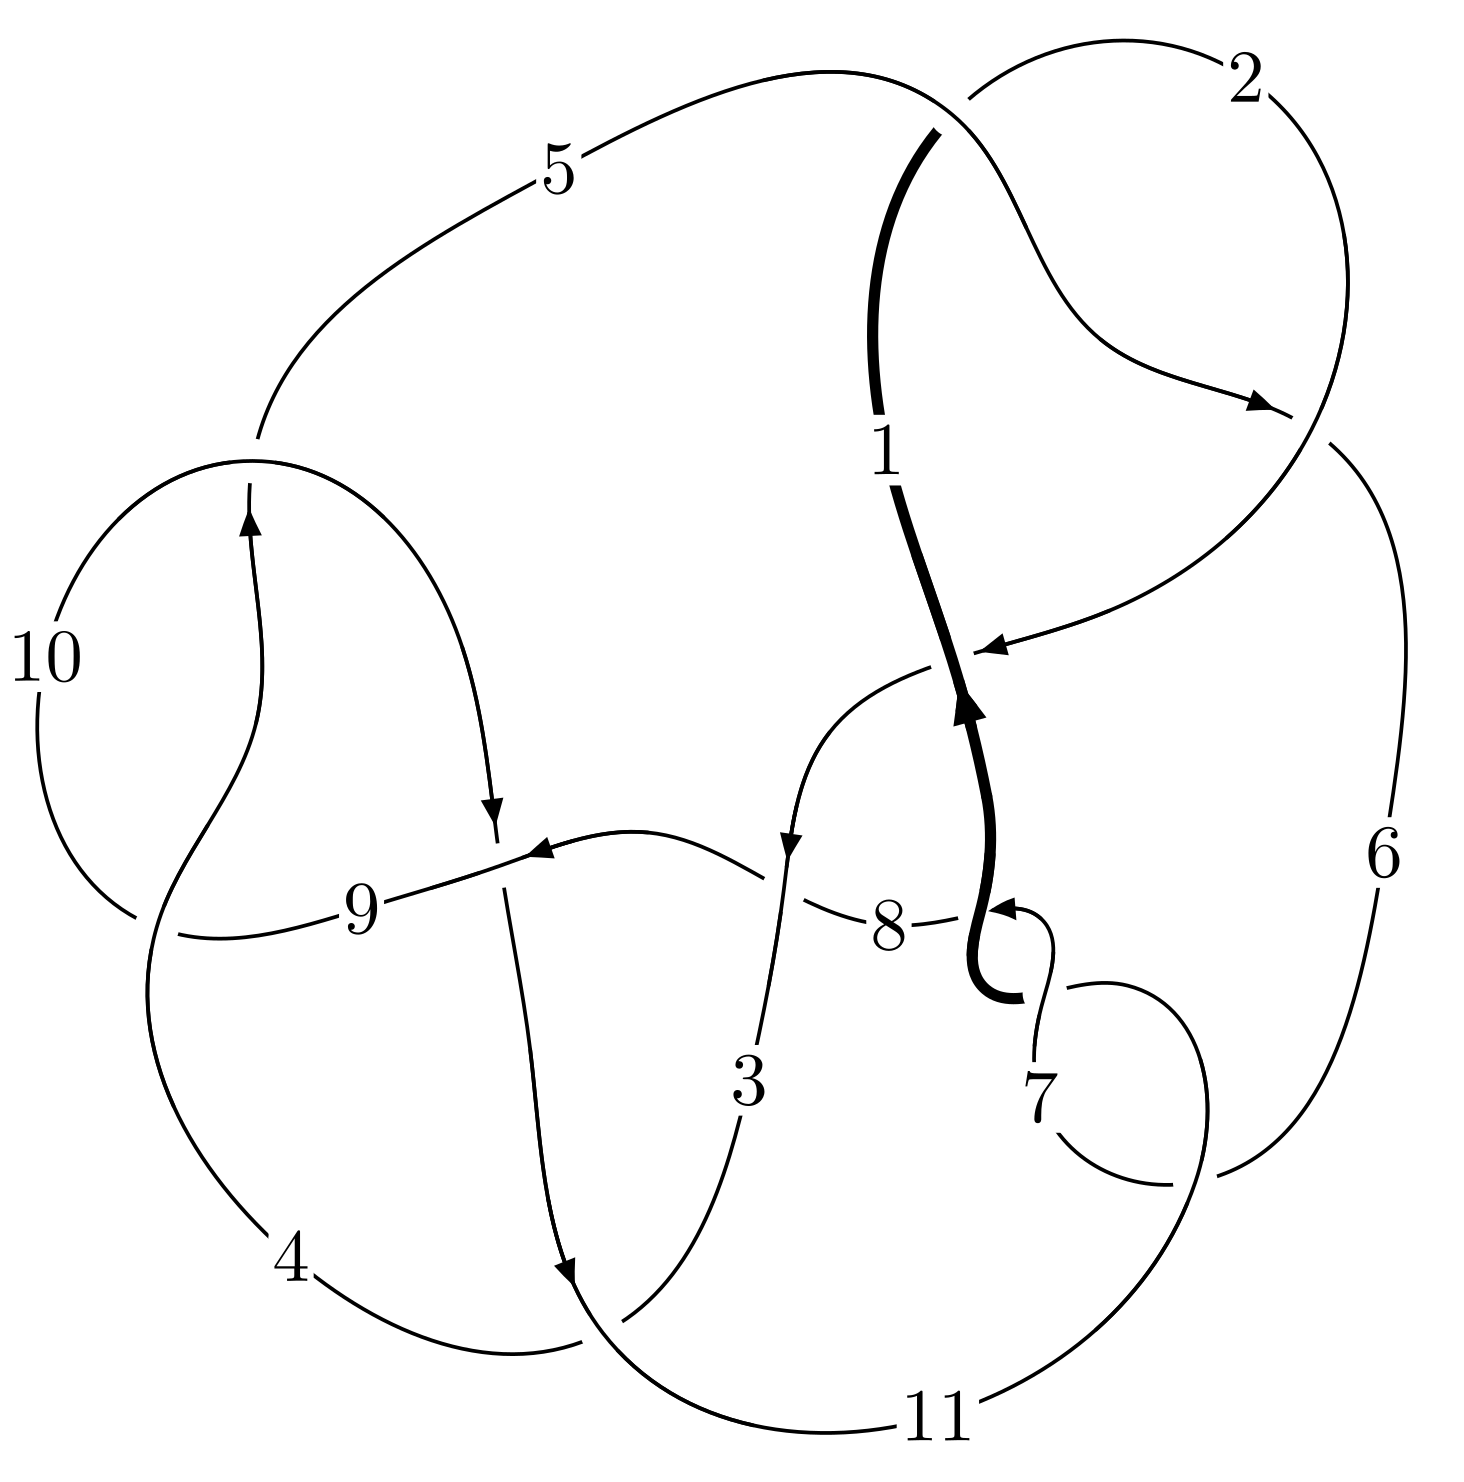
\includegraphics[width=112pt]{../../../GIT/diagram.site/Diagrams/png/721_11n_105.png}\\
\ \ \ A knot diagram\footnotemark}&
\allowdisplaybreaks
\textbf{Linearized knot diagam} \\
\cline{2-2}
 &
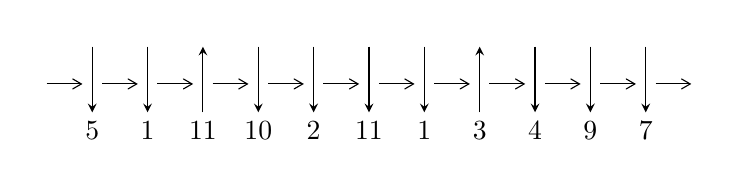
\begin{tikzpicture}[x=20pt, y=17pt]
	% nodes
	\node (C0) at (0, 0) {};
	\node (C1) at (1, 0) {};
	\node (C1U) at (1, +1) {};
	\node (C1D) at (1, -1) {5};

	\node (C2) at (2, 0) {};
	\node (C2U) at (2, +1) {};
	\node (C2D) at (2, -1) {1};

	\node (C3) at (3, 0) {};
	\node (C3U) at (3, +1) {};
	\node (C3D) at (3, -1) {11};

	\node (C4) at (4, 0) {};
	\node (C4U) at (4, +1) {};
	\node (C4D) at (4, -1) {10};

	\node (C5) at (5, 0) {};
	\node (C5U) at (5, +1) {};
	\node (C5D) at (5, -1) {2};

	\node (C6) at (6, 0) {};
	\node (C6U) at (6, +1) {};
	\node (C6D) at (6, -1) {11};

	\node (C7) at (7, 0) {};
	\node (C7U) at (7, +1) {};
	\node (C7D) at (7, -1) {1};

	\node (C8) at (8, 0) {};
	\node (C8U) at (8, +1) {};
	\node (C8D) at (8, -1) {3};

	\node (C9) at (9, 0) {};
	\node (C9U) at (9, +1) {};
	\node (C9D) at (9, -1) {4};

	\node (C10) at (10, 0) {};
	\node (C10U) at (10, +1) {};
	\node (C10D) at (10, -1) {9};

	\node (C11) at (11, 0) {};
	\node (C11U) at (11, +1) {};
	\node (C11D) at (11, -1) {7};
	\node (C12) at (12, 0) {};

	% arrows
	\draw[->,>={angle 60}]
	(C0) edge (C1) (C1) edge (C2) (C2) edge (C3) (C3) edge (C4) (C4) edge (C5) (C5) edge (C6) (C6) edge (C7) (C7) edge (C8) (C8) edge (C9) (C9) edge (C10) (C10) edge (C11) (C11) edge (C12) ;	\draw[->,>=stealth]
	(C1U) edge (C1D) (C2U) edge (C2D) (C3D) edge (C3U) (C4U) edge (C4D) (C5U) edge (C5D) (C6U) edge (C6D) (C7U) edge (C7D) (C8D) edge (C8U) (C9U) edge (C9D) (C10U) edge (C10D) (C11U) edge (C11D) ;
	\end{tikzpicture} \\
\hhline{~~} \\& 
\textbf{Solving Sequence} \\ \cline{2-2} 
 &
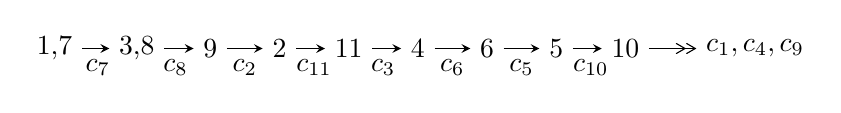
\begin{tikzpicture}[x=25pt, y=7pt]
	% node
	\node (A0) at (-1/8, 0) {1,7};
	\node (A1) at (17/16, 0) {3,8};
	\node (A2) at (17/8, 0) {9};
	\node (A3) at (25/8, 0) {2};
	\node (A4) at (33/8, 0) {11};
	\node (A5) at (41/8, 0) {4};
	\node (A6) at (49/8, 0) {6};
	\node (A7) at (57/8, 0) {5};
	\node (A8) at (65/8, 0) {10};
	\node (C1) at (1/2, -1) {$c_{7}$};
	\node (C2) at (13/8, -1) {$c_{8}$};
	\node (C3) at (21/8, -1) {$c_{2}$};
	\node (C4) at (29/8, -1) {$c_{11}$};
	\node (C5) at (37/8, -1) {$c_{3}$};
	\node (C6) at (45/8, -1) {$c_{6}$};
	\node (C7) at (53/8, -1) {$c_{5}$};
	\node (C8) at (61/8, -1) {$c_{10}$};
	\node (A9) at (10, 0) {$c_{1},c_{4},c_{9}$};

	% edge
	\draw[->,>=stealth]	
	(A0) edge (A1) (A1) edge (A2) (A2) edge (A3) (A3) edge (A4) (A4) edge (A5) (A5) edge (A6) (A6) edge (A7) (A7) edge (A8) ;
	\draw[->>,>={angle 60}]	
	(A8) edge (A9);
\end{tikzpicture} \\ 

\end{tabular} \\

\footnotetext{
The image of knot diagram is generated by the software ``\textbf{Draw programme}" developed by Andrew Bartholomew(\url{http://www.layer8.co.uk/maths/draw/index.htm\#Running-draw}), where we modified some parts for our purpose(\url{https://github.com/CATsTAILs/LinksPainter}).
}\phantom \\ \newline 
\centering \textbf{Ideals for irreducible components\footnotemark of $X_{\text{par}}$} 
 
\begin{align*}
I^u_{1}&=\langle 
- u^{17}+u^{16}+\cdots+8 b-1,\;a+u,\;u^{19}- u^{18}+\cdots+2 u-1\rangle \\
I^u_{2}&=\langle 
6724436 u^{21}-6900373 u^{20}+\cdots+11494529 b-7797736,\\
\phantom{I^u_{2}}&\phantom{= \langle  }3098806 u^{21}+3180019 u^{20}+\cdots+57472645 a+15394503,\;u^{22}- u^{21}+\cdots-2 u+5\rangle \\
I^u_{3}&=\langle 
b^4-4 b^3+8 b^2-8 b+5,\;a-1,\;u+1\rangle \\
I^u_{4}&=\langle 
b^3+3 b^2+3 b+1,\;a+1,\;u-1\rangle \\
\\
\end{align*}
\raggedright * 4 irreducible components of $\dim_{\mathbb{C}}=0$, with total 48 representations.\\
\footnotetext{All coefficients of polynomials are rational numbers. But the coefficients are sometimes approximated in decimal forms when there is not enough margin.}
\newpage
\renewcommand{\arraystretch}{1}
\centering \section*{I. $I^u_{1}= \langle - u^{17}+u^{16}+\cdots+8 b-1,\;a+u,\;u^{19}- u^{18}+\cdots+2 u-1 \rangle$}
\flushleft \textbf{(i) Arc colorings}\\
\begin{tabular}{m{7pt} m{180pt} m{7pt} m{180pt} }
\flushright $a_{1}=$&$\begin{pmatrix}0\\u\end{pmatrix}$ \\
\flushright $a_{7}=$&$\begin{pmatrix}1\\0\end{pmatrix}$ \\
\flushright $a_{3}=$&$\begin{pmatrix}- u\\\frac{1}{8} u^{17}-\frac{1}{8} u^{16}+\cdots+\frac{3}{4} u+\frac{1}{8}\end{pmatrix}$ \\
\flushright $a_{8}=$&$\begin{pmatrix}1\\u^2\end{pmatrix}$ \\
\flushright $a_{9}=$&$\begin{pmatrix}\frac{1}{8} u^{18}-\frac{1}{8} u^{17}+\cdots+\frac{1}{8} u+1\\-\frac{3}{4} u^{18}+\frac{7}{8} u^{17}+\cdots-\frac{5}{4} u+\frac{1}{8}\end{pmatrix}$ \\
\flushright $a_{2}=$&$\begin{pmatrix}- u\\\frac{1}{8} u^{17}-\frac{1}{8} u^{16}+\cdots+\frac{3}{4} u+\frac{1}{8}\end{pmatrix}$ \\
\flushright $a_{11}=$&$\begin{pmatrix}u\\u\end{pmatrix}$ \\
\flushright $a_{4}=$&$\begin{pmatrix}\frac{1}{8} u^{17}-\frac{1}{8} u^{16}+\cdots-\frac{5}{4} u+\frac{1}{8}\\\frac{1}{4} u^{17}-\frac{1}{4} u^{16}+\cdots+\frac{1}{2} u+\frac{1}{4}\end{pmatrix}$ \\
\flushright $a_{6}=$&$\begin{pmatrix}- u^2+1\\- u^2\end{pmatrix}$ \\
\flushright $a_{5}=$&$\begin{pmatrix}1\\-\frac{1}{8} u^{18}+\frac{1}{8} u^{17}+\cdots-\frac{7}{4} u^2-\frac{1}{8} u\end{pmatrix}$ \\
\flushright $a_{10}=$&$\begin{pmatrix}-\frac{1}{2} u^{18}+\frac{9}{8} u^{17}+\cdots-\frac{5}{2} u+\frac{15}{8}\\-\frac{7}{8} u^{18}+\frac{17}{8} u^{17}+\cdots-\frac{9}{8} u+1\end{pmatrix}$\\ \flushright $a_{10}=$&$\begin{pmatrix}-\frac{1}{2} u^{18}+\frac{9}{8} u^{17}+\cdots-\frac{5}{2} u+\frac{15}{8}\\-\frac{7}{8} u^{18}+\frac{17}{8} u^{17}+\cdots-\frac{9}{8} u+1\end{pmatrix}$\\&\end{tabular}
\flushleft \textbf{(ii) Obstruction class $= -1$}\\~\\
\flushleft \textbf{(iii) Cusp Shapes $= -\frac{5}{2} u^{18}+\frac{11}{4} u^{17}+\frac{15}{4} u^{16}-\frac{25}{4} u^{15}-\frac{37}{2} u^{14}+\frac{93}{4} u^{13}+\frac{27}{2} u^{12}-\frac{123}{4} u^{11}-\frac{139}{4} u^{10}+\frac{191}{4} u^9+\frac{21}{4} u^8-\frac{135}{4} u^7-\frac{41}{4} u^6+\frac{55}{4} u^5-\frac{21}{4} u^4-\frac{17}{4} u^3+8 u^2+\frac{7}{2} u-\frac{53}{4}$}\\~\\
\newpage\renewcommand{\arraystretch}{1}
\flushleft \textbf{(iv) u-Polynomials at the component}\newline \\
\begin{tabular}{m{50pt}|m{274pt}}
Crossings & \hspace{64pt}u-Polynomials at each crossing \\
\hline $$\begin{aligned}c_{1},c_{5},c_{6}\\c_{7},c_{11}\end{aligned}$$&$\begin{aligned}
&u^{19}+u^{18}+\cdots+2 u+1
\end{aligned}$\\
\hline $$\begin{aligned}c_{2}\end{aligned}$$&$\begin{aligned}
&u^{19}+5 u^{18}+\cdots+10 u+1
\end{aligned}$\\
\hline $$\begin{aligned}c_{3}\end{aligned}$$&$\begin{aligned}
&u^{19}+9 u^{18}+\cdots+106 u+14
\end{aligned}$\\
\hline $$\begin{aligned}c_{4},c_{9}\end{aligned}$$&$\begin{aligned}
&u^{19}+3 u^{18}+\cdots+6 u+2
\end{aligned}$\\
\hline $$\begin{aligned}c_{8}\end{aligned}$$&$\begin{aligned}
&u^{19}-3 u^{18}+\cdots-70 u+26
\end{aligned}$\\
\hline $$\begin{aligned}c_{10}\end{aligned}$$&$\begin{aligned}
&u^{19}+9 u^{18}+\cdots+4 u+4
\end{aligned}$\\
\hline
\end{tabular}\\~\\
\newpage\renewcommand{\arraystretch}{1}
\flushleft \textbf{(v) Riley Polynomials at the component}\newline \\
\begin{tabular}{m{50pt}|m{274pt}}
Crossings & \hspace{64pt}Riley Polynomials at each crossing \\
\hline $$\begin{aligned}c_{1},c_{5},c_{6}\\c_{7},c_{11}\end{aligned}$$&$\begin{aligned}
&y^{19}-5 y^{18}+\cdots+10 y-1
\end{aligned}$\\
\hline $$\begin{aligned}c_{2}\end{aligned}$$&$\begin{aligned}
&y^{19}+27 y^{18}+\cdots+38 y-1
\end{aligned}$\\
\hline $$\begin{aligned}c_{3}\end{aligned}$$&$\begin{aligned}
&y^{19}+3 y^{18}+\cdots+1044 y-196
\end{aligned}$\\
\hline $$\begin{aligned}c_{4},c_{9}\end{aligned}$$&$\begin{aligned}
&y^{19}-9 y^{18}+\cdots+4 y-4
\end{aligned}$\\
\hline $$\begin{aligned}c_{8}\end{aligned}$$&$\begin{aligned}
&y^{19}-9 y^{18}+\cdots-14444 y-676
\end{aligned}$\\
\hline $$\begin{aligned}c_{10}\end{aligned}$$&$\begin{aligned}
&y^{19}+3 y^{18}+\cdots+144 y-16
\end{aligned}$\\
\hline
\end{tabular}\\~\\
\newpage\flushleft \textbf{(vi) Complex Volumes and Cusp Shapes}
$$\begin{array}{c|c|c}  
\text{Solutions to }I^u_{1}& \I (\text{vol} + \sqrt{-1}CS) & \text{Cusp shape}\\
 \hline 
\begin{aligned}
u &= -0.777977 + 0.409956 I \\
a &= \phantom{-}0.777977 - 0.409956 I \\
b &= \phantom{-}0.369181 + 0.923791 I\end{aligned}
 & -4.54946 + 5.47873 I & -11.07465 - 8.55667 I \\ \hline\begin{aligned}
u &= -0.777977 - 0.409956 I \\
a &= \phantom{-}0.777977 + 0.409956 I \\
b &= \phantom{-}0.369181 - 0.923791 I\end{aligned}
 & -4.54946 - 5.47873 I & -11.07465 + 8.55667 I \\ \hline\begin{aligned}
u &= \phantom{-}0.133918 + 0.761043 I \\
a &= -0.133918 - 0.761043 I \\
b &= \phantom{-}0.139898 + 0.619393 I\end{aligned}
 & \phantom{-}1.53985 - 2.22177 I & -2.53368 + 4.26379 I \\ \hline\begin{aligned}
u &= \phantom{-}0.133918 - 0.761043 I \\
a &= -0.133918 + 0.761043 I \\
b &= \phantom{-}0.139898 - 0.619393 I\end{aligned}
 & \phantom{-}1.53985 + 2.22177 I & -2.53368 - 4.26379 I \\ \hline\begin{aligned}
u &= \phantom{-}0.647319 + 0.397441 I \\
a &= -0.647319 - 0.397441 I \\
b &= \phantom{-}0.063657 + 0.711783 I\end{aligned}
 & -1.23847 - 1.46671 I & -6.68531 + 4.74531 I \\ \hline\begin{aligned}
u &= \phantom{-}0.647319 - 0.397441 I \\
a &= -0.647319 + 0.397441 I \\
b &= \phantom{-}0.063657 - 0.711783 I\end{aligned}
 & -1.23847 + 1.46671 I & -6.68531 - 4.74531 I \\ \hline\begin{aligned}
u &= -0.697477 + 0.278835 I \\
a &= \phantom{-}0.697477 - 0.278835 I \\
b &= -0.339503 + 1.077420 I\end{aligned}
 & -4.36768 - 2.62850 I & -9.97134 - 1.16882 I \\ \hline\begin{aligned}
u &= -0.697477 - 0.278835 I \\
a &= \phantom{-}0.697477 + 0.278835 I \\
b &= -0.339503 - 1.077420 I\end{aligned}
 & -4.36768 + 2.62850 I & -9.97134 + 1.16882 I \\ \hline\begin{aligned}
u &= \phantom{-}1.033800 + 0.730109 I \\
a &= -1.033800 - 0.730109 I \\
b &= -0.98428 - 1.15874 I\end{aligned}
 & -0.86154 - 5.74817 I & -11.63360 + 4.50327 I \\ \hline\begin{aligned}
u &= \phantom{-}1.033800 - 0.730109 I \\
a &= -1.033800 + 0.730109 I \\
b &= -0.98428 + 1.15874 I\end{aligned}
 & -0.86154 + 5.74817 I & -11.63360 - 4.50327 I\\
 \hline 
 \end{array}$$\newpage$$\begin{array}{c|c|c}  
\text{Solutions to }I^u_{1}& \I (\text{vol} + \sqrt{-1}CS) & \text{Cusp shape}\\
 \hline 
\begin{aligned}
u &= \phantom{-}0.887480 + 0.926590 I \\
a &= -0.887480 - 0.926590 I \\
b &= \phantom{-}0.401639 - 1.047330 I\end{aligned}
 & \phantom{-}4.22972 + 0.35072 I & -6.13837 - 0.22490 I \\ \hline\begin{aligned}
u &= \phantom{-}0.887480 - 0.926590 I \\
a &= -0.887480 + 0.926590 I \\
b &= \phantom{-}0.401639 + 1.047330 I\end{aligned}
 & \phantom{-}4.22972 - 0.35072 I & -6.13837 + 0.22490 I \\ \hline\begin{aligned}
u &= -0.968832 + 0.893275 I \\
a &= \phantom{-}0.968832 - 0.893275 I \\
b &= -0.058802 - 1.386650 I\end{aligned}
 & \phantom{-}5.51436 + 5.01792 I & -4.62542 - 4.88249 I \\ \hline\begin{aligned}
u &= -0.968832 - 0.893275 I \\
a &= \phantom{-}0.968832 + 0.893275 I \\
b &= -0.058802 + 1.386650 I\end{aligned}
 & \phantom{-}5.51436 - 5.01792 I & -4.62542 + 4.88249 I \\ \hline\begin{aligned}
u &= -1.107490 + 0.812678 I \\
a &= \phantom{-}1.107490 - 0.812678 I \\
b &= \phantom{-}0.84460 - 1.89768 I\end{aligned}
 & \phantom{-}4.47255 + 8.26447 I & -5.93446 - 4.83162 I \\ \hline\begin{aligned}
u &= -1.107490 - 0.812678 I \\
a &= \phantom{-}1.107490 + 0.812678 I \\
b &= \phantom{-}0.84460 + 1.89768 I\end{aligned}
 & \phantom{-}4.47255 - 8.26447 I & -5.93446 + 4.83162 I \\ \hline\begin{aligned}
u &= \phantom{-}1.151650 + 0.788448 I \\
a &= -1.151650 - 0.788448 I \\
b &= -1.17629 - 2.06224 I\end{aligned}
 & \phantom{-}2.31925 - 13.64210 I & -8.92588 + 8.81475 I \\ \hline\begin{aligned}
u &= \phantom{-}1.151650 - 0.788448 I \\
a &= -1.151650 + 0.788448 I \\
b &= -1.17629 + 2.06224 I\end{aligned}
 & \phantom{-}2.31925 + 13.64210 I & -8.92588 - 8.81475 I \\ \hline\begin{aligned}
u &= \phantom{-}0.395222\phantom{ +0.000000I} \\
a &= -0.395222\phantom{ +0.000000I} \\
b &= \phantom{-}0.479812\phantom{ +0.000000I}\end{aligned}
 & -0.957690\phantom{ +0.000000I} & -10.9550\phantom{ +0.000000I}\\
 \hline 
 \end{array}$$\newpage\newpage\renewcommand{\arraystretch}{1}
\centering \section*{II. $I^u_{2}= \langle 6.72\times10^{6} u^{21}-6.90\times10^{6} u^{20}+\cdots+1.15\times10^{7} b-7.80\times10^{6},\;3.10\times10^{6} u^{21}+3.18\times10^{6} u^{20}+\cdots+5.75\times10^{7} a+1.54\times10^{7},\;u^{22}- u^{21}+\cdots-2 u+5 \rangle$}
\flushleft \textbf{(i) Arc colorings}\\
\begin{tabular}{m{7pt} m{180pt} m{7pt} m{180pt} }
\flushright $a_{1}=$&$\begin{pmatrix}0\\u\end{pmatrix}$ \\
\flushright $a_{7}=$&$\begin{pmatrix}1\\0\end{pmatrix}$ \\
\flushright $a_{3}=$&$\begin{pmatrix}-0.0539179 u^{21}-0.0553310 u^{20}+\cdots-5.96818 u-0.267858\\-0.585012 u^{21}+0.600318 u^{20}+\cdots-1.51708 u+0.678387\end{pmatrix}$ \\
\flushright $a_{8}=$&$\begin{pmatrix}1\\u^2\end{pmatrix}$ \\
\flushright $a_{9}=$&$\begin{pmatrix}0.0828205 u^{21}-0.00564449 u^{20}+\cdots+0.238599 u-2.78491\\-0.124555 u^{21}+0.416476 u^{20}+\cdots+0.115943 u-2.65547\end{pmatrix}$ \\
\flushright $a_{2}=$&$\begin{pmatrix}-0.0539179 u^{21}-0.0553310 u^{20}+\cdots-5.96818 u-0.267858\\-0.253918 u^{21}+0.144669 u^{20}+\cdots-1.56818 u+0.132142\end{pmatrix}$ \\
\flushright $a_{11}=$&$\begin{pmatrix}u\\u\end{pmatrix}$ \\
\flushright $a_{4}=$&$\begin{pmatrix}-0.345839 u^{21}+0.500433 u^{20}+\cdots-3.06360 u-0.890633\\-0.876933 u^{21}+1.15608 u^{20}+\cdots+1.38750 u+0.0556113\end{pmatrix}$ \\
\flushright $a_{6}=$&$\begin{pmatrix}- u^2+1\\- u^2\end{pmatrix}$ \\
\flushright $a_{5}=$&$\begin{pmatrix}-0.0264284 u^{21}-0.227490 u^{20}+\cdots-0.137095 u-2.51532\\-1\end{pmatrix}$ \\
\flushright $a_{10}=$&$\begin{pmatrix}-0.628809 u^{21}+0.408950 u^{20}+\cdots-0.851245 u-1.74742\\-1.23704 u^{21}+1.45113 u^{20}+\cdots+3.35522 u+0.270710\end{pmatrix}$\\ \flushright $a_{10}=$&$\begin{pmatrix}-0.628809 u^{21}+0.408950 u^{20}+\cdots-0.851245 u-1.74742\\-1.23704 u^{21}+1.45113 u^{20}+\cdots+3.35522 u+0.270710\end{pmatrix}$\\&\end{tabular}
\flushleft \textbf{(ii) Obstruction class $= -1$}\\~\\
\flushleft \textbf{(iii) Cusp Shapes $= \frac{492576}{11494529} u^{21}+\frac{21062536}{11494529} u^{20}+\cdots-\frac{92150964}{11494529} u-\frac{289179942}{11494529}$}\\~\\
\newpage\renewcommand{\arraystretch}{1}
\flushleft \textbf{(iv) u-Polynomials at the component}\newline \\
\begin{tabular}{m{50pt}|m{274pt}}
Crossings & \hspace{64pt}u-Polynomials at each crossing \\
\hline $$\begin{aligned}c_{1},c_{5},c_{6}\\c_{7},c_{11}\end{aligned}$$&$\begin{aligned}
&u^{22}+u^{21}+\cdots+2 u+5
\end{aligned}$\\
\hline $$\begin{aligned}c_{2}\end{aligned}$$&$\begin{aligned}
&u^{22}+9 u^{21}+\cdots+224 u+25
\end{aligned}$\\
\hline $$\begin{aligned}c_{3}\end{aligned}$$&$\begin{aligned}
&(u^{11}-3 u^{10}+4 u^9- u^8+2 u^7-8 u^6+8 u^5+5 u^4-3 u^3- u^2+4 u-1)^2
\end{aligned}$\\
\hline $$\begin{aligned}c_{4},c_{9}\end{aligned}$$&$\begin{aligned}
&(u^{11}- u^{10}-2 u^9+3 u^8+2 u^7-4 u^6+3 u^4- u^3- u^2+1)^2
\end{aligned}$\\
\hline $$\begin{aligned}c_{8}\end{aligned}$$&$\begin{aligned}
&(u^{11}+u^{10}-6 u^9-5 u^8+12 u^7+6 u^6-10 u^5+u^4+5 u^3- u^2+1)^2
\end{aligned}$\\
\hline $$\begin{aligned}c_{10}\end{aligned}$$&$\begin{aligned}
&(u^{11}+5 u^{10}+\cdots+2 u+1)^{2}
\end{aligned}$\\
\hline
\end{tabular}\\~\\
\newpage\renewcommand{\arraystretch}{1}
\flushleft \textbf{(v) Riley Polynomials at the component}\newline \\
\begin{tabular}{m{50pt}|m{274pt}}
Crossings & \hspace{64pt}Riley Polynomials at each crossing \\
\hline $$\begin{aligned}c_{1},c_{5},c_{6}\\c_{7},c_{11}\end{aligned}$$&$\begin{aligned}
&y^{22}-9 y^{21}+\cdots-224 y+25
\end{aligned}$\\
\hline $$\begin{aligned}c_{2}\end{aligned}$$&$\begin{aligned}
&y^{22}+7 y^{21}+\cdots+5624 y+625
\end{aligned}$\\
\hline $$\begin{aligned}c_{3}\end{aligned}$$&$\begin{aligned}
&(y^{11}- y^{10}+\cdots+14 y-1)^{2}
\end{aligned}$\\
\hline $$\begin{aligned}c_{4},c_{9}\end{aligned}$$&$\begin{aligned}
&(y^{11}-5 y^{10}+\cdots+2 y-1)^{2}
\end{aligned}$\\
\hline $$\begin{aligned}c_{8}\end{aligned}$$&$\begin{aligned}
&(y^{11}-13 y^{10}+\cdots+2 y-1)^{2}
\end{aligned}$\\
\hline $$\begin{aligned}c_{10}\end{aligned}$$&$\begin{aligned}
&(y^{11}+3 y^{10}+\cdots-10 y-1)^{2}
\end{aligned}$\\
\hline
\end{tabular}\\~\\
\newpage\flushleft \textbf{(vi) Complex Volumes and Cusp Shapes}
$$\begin{array}{c|c|c}  
\text{Solutions to }I^u_{2}& \I (\text{vol} + \sqrt{-1}CS) & \text{Cusp shape}\\
 \hline 
\begin{aligned}
u &= \phantom{-}0.968725 + 0.342171 I \\
a &= -1.14483 + 0.84471 I \\
b &= -1.72734 + 0.45538 I\end{aligned}
 & -4.92613 + 1.27541 I & -13.47945 - 0.80097 I \\ \hline\begin{aligned}
u &= \phantom{-}0.968725 - 0.342171 I \\
a &= -1.14483 - 0.84471 I \\
b &= -1.72734 - 0.45538 I\end{aligned}
 & -4.92613 - 1.27541 I & -13.47945 + 0.80097 I \\ \hline\begin{aligned}
u &= \phantom{-}0.729583 + 0.772577 I \\
a &= \phantom{-}0.813042 + 0.684201 I \\
b &= \phantom{-}0.635345 + 0.872369 I\end{aligned}
 & \phantom{-}0.0927065\phantom{ +0.000000I} & -9.81428 + 0. I\phantom{ +0.000000I} \\ \hline\begin{aligned}
u &= \phantom{-}0.729583 - 0.772577 I \\
a &= \phantom{-}0.813042 - 0.684201 I \\
b &= \phantom{-}0.635345 - 0.872369 I\end{aligned}
 & \phantom{-}0.0927065\phantom{ +0.000000I} & -9.81428 + 0. I\phantom{ +0.000000I} \\ \hline\begin{aligned}
u &= \phantom{-}1.182920 + 0.018546 I \\
a &= -0.183030 - 0.210319 I \\
b &= \phantom{-}0.415301 - 0.525828 I\end{aligned}
 & -1.99990 - 0.45477 I & -4.80492 + 1.36957 I \\ \hline\begin{aligned}
u &= \phantom{-}1.182920 - 0.018546 I \\
a &= -0.183030 + 0.210319 I \\
b &= \phantom{-}0.415301 + 0.525828 I\end{aligned}
 & -1.99990 + 0.45477 I & -4.80492 - 1.36957 I \\ \hline\begin{aligned}
u &= \phantom{-}0.624756 + 1.026890 I \\
a &= \phantom{-}1.16034 + 0.84838 I \\
b &= -0.266486 + 1.063010 I\end{aligned}
 & \phantom{-}3.97498 + 7.02220 I & -6.49946 - 4.88619 I \\ \hline\begin{aligned}
u &= \phantom{-}0.624756 - 1.026890 I \\
a &= \phantom{-}1.16034 - 0.84838 I \\
b &= -0.266486 - 1.063010 I\end{aligned}
 & \phantom{-}3.97498 - 7.02220 I & -6.49946 + 4.88619 I \\ \hline\begin{aligned}
u &= -1.195770 + 0.178364 I \\
a &= \phantom{-}0.591030 + 0.642561 I \\
b &= \phantom{-}0.87334 + 1.16676 I\end{aligned}
 & -4.92613 + 1.27541 I & -13.47945 - 0.80097 I \\ \hline\begin{aligned}
u &= -1.195770 - 0.178364 I \\
a &= \phantom{-}0.591030 - 0.642561 I \\
b &= \phantom{-}0.87334 - 1.16676 I\end{aligned}
 & -4.92613 - 1.27541 I & -13.47945 + 0.80097 I\\
 \hline 
 \end{array}$$\newpage$$\begin{array}{c|c|c}  
\text{Solutions to }I^u_{2}& \I (\text{vol} + \sqrt{-1}CS) & \text{Cusp shape}\\
 \hline 
\begin{aligned}
u &= \phantom{-}0.620308 + 0.489049 I \\
a &= -1.65639 + 1.26230 I \\
b &= -1.66929 - 0.34266 I\end{aligned}
 & -3.66655 - 4.75030 I & -9.35891 + 6.77690 I \\ \hline\begin{aligned}
u &= \phantom{-}0.620308 - 0.489049 I \\
a &= -1.65639 - 1.26230 I \\
b &= -1.66929 + 0.34266 I\end{aligned}
 & -3.66655 + 4.75030 I & -9.35891 - 6.77690 I \\ \hline\begin{aligned}
u &= -0.703026 + 0.993334 I \\
a &= -1.120470 + 0.746267 I \\
b &= -0.001089 + 1.272950 I\end{aligned}
 & \phantom{-}5.74879 - 1.64593 I & -3.95012 + 0.24481 I \\ \hline\begin{aligned}
u &= -0.703026 - 0.993334 I \\
a &= -1.120470 - 0.746267 I \\
b &= -0.001089 - 1.272950 I\end{aligned}
 & \phantom{-}5.74879 + 1.64593 I & -3.95012 - 0.24481 I \\ \hline\begin{aligned}
u &= -0.892154 + 0.917804 I \\
a &= -1.050620 + 0.484687 I \\
b &= -0.75266 + 1.62251 I\end{aligned}
 & \phantom{-}5.74879 + 1.64593 I & -3.95012 - 0.24481 I \\ \hline\begin{aligned}
u &= -0.892154 - 0.917804 I \\
a &= -1.050620 - 0.484687 I \\
b &= -0.75266 - 1.62251 I\end{aligned}
 & \phantom{-}5.74879 - 1.64593 I & -3.95012 + 0.24481 I \\ \hline\begin{aligned}
u &= -1.282540 + 0.010543 I \\
a &= \phantom{-}0.117415 - 0.472097 I \\
b &= -0.481877 - 1.258190 I\end{aligned}
 & -3.66655 + 4.75030 I & -9.35891 - 6.77690 I \\ \hline\begin{aligned}
u &= -1.282540 - 0.010543 I \\
a &= \phantom{-}0.117415 + 0.472097 I \\
b &= -0.481877 + 1.258190 I\end{aligned}
 & -3.66655 - 4.75030 I & -9.35891 + 6.77690 I \\ \hline\begin{aligned}
u &= \phantom{-}0.967997 + 0.889244 I \\
a &= \phantom{-}1.032500 + 0.377033 I \\
b &= \phantom{-}1.09468 + 1.69502 I\end{aligned}
 & \phantom{-}3.97498 - 7.02220 I & -6.49946 + 4.88619 I \\ \hline\begin{aligned}
u &= \phantom{-}0.967997 - 0.889244 I \\
a &= \phantom{-}1.032500 - 0.377033 I \\
b &= \phantom{-}1.09468 - 1.69502 I\end{aligned}
 & \phantom{-}3.97498 + 7.02220 I & -6.49946 - 4.88619 I\\
 \hline 
 \end{array}$$\newpage$$\begin{array}{c|c|c}  
\text{Solutions to }I^u_{2}& \I (\text{vol} + \sqrt{-1}CS) & \text{Cusp shape}\\
 \hline 
\begin{aligned}
u &= -0.520797 + 0.242115 I \\
a &= \phantom{-}2.24102 + 0.95759 I \\
b &= \phantom{-}1.380080 - 0.137991 I\end{aligned}
 & -1.99990 + 0.45477 I & -4.80492 - 1.36957 I \\ \hline\begin{aligned}
u &= -0.520797 - 0.242115 I \\
a &= \phantom{-}2.24102 - 0.95759 I \\
b &= \phantom{-}1.380080 + 0.137991 I\end{aligned}
 & -1.99990 - 0.45477 I & -4.80492 + 1.36957 I\\
 \hline 
 \end{array}$$\newpage\newpage\renewcommand{\arraystretch}{1}
\centering \section*{III. $I^u_{3}= \langle b^4-4 b^3+8 b^2-8 b+5,\;a-1,\;u+1 \rangle$}
\flushleft \textbf{(i) Arc colorings}\\
\begin{tabular}{m{7pt} m{180pt} m{7pt} m{180pt} }
\flushright $a_{1}=$&$\begin{pmatrix}0\\-1\end{pmatrix}$ \\
\flushright $a_{7}=$&$\begin{pmatrix}1\\0\end{pmatrix}$ \\
\flushright $a_{3}=$&$\begin{pmatrix}1\\b\end{pmatrix}$ \\
\flushright $a_{8}=$&$\begin{pmatrix}1\\1\end{pmatrix}$ \\
\flushright $a_{9}=$&$\begin{pmatrix}- b+2\\- b^2+b+1\end{pmatrix}$ \\
\flushright $a_{2}=$&$\begin{pmatrix}1\\b-1\end{pmatrix}$ \\
\flushright $a_{11}=$&$\begin{pmatrix}-1\\-1\end{pmatrix}$ \\
\flushright $a_{4}=$&$\begin{pmatrix}b\\2 b-1\end{pmatrix}$ \\
\flushright $a_{6}=$&$\begin{pmatrix}0\\-1\end{pmatrix}$ \\
\flushright $a_{5}=$&$\begin{pmatrix}-1\\- b\end{pmatrix}$ \\
\flushright $a_{10}=$&$\begin{pmatrix}b^3-4 b^2+5 b-3\\b^3-6 b^2+9 b-7\end{pmatrix}$\\ \flushright $a_{10}=$&$\begin{pmatrix}b^3-4 b^2+5 b-3\\b^3-6 b^2+9 b-7\end{pmatrix}$\\&\end{tabular}
\flushleft \textbf{(ii) Obstruction class $= 1$}\\~\\
\flushleft \textbf{(iii) Cusp Shapes $= -4 b^2+8 b-24$}\\~\\
\newpage\renewcommand{\arraystretch}{1}
\flushleft \textbf{(iv) u-Polynomials at the component}\newline \\
\begin{tabular}{m{50pt}|m{274pt}}
Crossings & \hspace{64pt}u-Polynomials at each crossing \\
\hline $$\begin{aligned}c_{1},c_{2},c_{6}\\c_{7}\end{aligned}$$&$\begin{aligned}
&(u+1)^4
\end{aligned}$\\
\hline $$\begin{aligned}c_{3},c_{8}\end{aligned}$$&$\begin{aligned}
&u^4+2 u^2+2
\end{aligned}$\\
\hline $$\begin{aligned}c_{4},c_{9}\end{aligned}$$&$\begin{aligned}
&u^4-2 u^2+2
\end{aligned}$\\
\hline $$\begin{aligned}c_{5},c_{11}\end{aligned}$$&$\begin{aligned}
&(u-1)^4
\end{aligned}$\\
\hline $$\begin{aligned}c_{10}\end{aligned}$$&$\begin{aligned}
&(u^2+2 u+2)^2
\end{aligned}$\\
\hline
\end{tabular}\\~\\
\newpage\renewcommand{\arraystretch}{1}
\flushleft \textbf{(v) Riley Polynomials at the component}\newline \\
\begin{tabular}{m{50pt}|m{274pt}}
Crossings & \hspace{64pt}Riley Polynomials at each crossing \\
\hline $$\begin{aligned}c_{1},c_{2},c_{5}\\c_{6},c_{7},c_{11}\end{aligned}$$&$\begin{aligned}
&(y-1)^4
\end{aligned}$\\
\hline $$\begin{aligned}c_{3},c_{8}\end{aligned}$$&$\begin{aligned}
&(y^2+2 y+2)^2
\end{aligned}$\\
\hline $$\begin{aligned}c_{4},c_{9}\end{aligned}$$&$\begin{aligned}
&(y^2-2 y+2)^2
\end{aligned}$\\
\hline $$\begin{aligned}c_{10}\end{aligned}$$&$\begin{aligned}
&(y^2+4)^2
\end{aligned}$\\
\hline
\end{tabular}\\~\\
\newpage\flushleft \textbf{(vi) Complex Volumes and Cusp Shapes}
$$\begin{array}{c|c|c}  
\text{Solutions to }I^u_{3}& \I (\text{vol} + \sqrt{-1}CS) & \text{Cusp shape}\\
 \hline 
\begin{aligned}
u &= -1.00000\phantom{ +0.000000I} \\
a &= \phantom{-}1.00000\phantom{ +0.000000I} \\
b &= \phantom{-}0.544910 + 1.098680 I\end{aligned}
 & -5.75727 - 3.66386 I & -16.0000 + 4.0000 I \\ \hline\begin{aligned}
u &= -1.00000\phantom{ +0.000000I} \\
a &= \phantom{-}1.00000\phantom{ +0.000000I} \\
b &= \phantom{-}0.544910 - 1.098680 I\end{aligned}
 & -5.75727 + 3.66386 I & -16.0000 - 4.0000 I \\ \hline\begin{aligned}
u &= -1.00000\phantom{ +0.000000I} \\
a &= \phantom{-}1.00000\phantom{ +0.000000I} \\
b &= \phantom{-}1.45509 + 1.09868 I\end{aligned}
 & -5.75727 + 3.66386 I & -16.0000 - 4.0000 I \\ \hline\begin{aligned}
u &= -1.00000\phantom{ +0.000000I} \\
a &= \phantom{-}1.00000\phantom{ +0.000000I} \\
b &= \phantom{-}1.45509 - 1.09868 I\end{aligned}
 & -5.75727 - 3.66386 I & -16.0000 + 4.0000 I\\
 \hline 
 \end{array}$$\newpage\newpage\renewcommand{\arraystretch}{1}
\centering \section*{IV. $I^u_{4}= \langle b^3+3 b^2+3 b+1,\;a+1,\;u-1 \rangle$}
\flushleft \textbf{(i) Arc colorings}\\
\begin{tabular}{m{7pt} m{180pt} m{7pt} m{180pt} }
\flushright $a_{1}=$&$\begin{pmatrix}0\\1\end{pmatrix}$ \\
\flushright $a_{7}=$&$\begin{pmatrix}1\\0\end{pmatrix}$ \\
\flushright $a_{3}=$&$\begin{pmatrix}-1\\b\end{pmatrix}$ \\
\flushright $a_{8}=$&$\begin{pmatrix}1\\1\end{pmatrix}$ \\
\flushright $a_{9}=$&$\begin{pmatrix}b+2\\- b^2- b+1\end{pmatrix}$ \\
\flushright $a_{2}=$&$\begin{pmatrix}-1\\b+1\end{pmatrix}$ \\
\flushright $a_{11}=$&$\begin{pmatrix}1\\1\end{pmatrix}$ \\
\flushright $a_{4}=$&$\begin{pmatrix}b\\2 b+1\end{pmatrix}$ \\
\flushright $a_{6}=$&$\begin{pmatrix}0\\-1\end{pmatrix}$ \\
\flushright $a_{5}=$&$\begin{pmatrix}-1\\b\end{pmatrix}$ \\
\flushright $a_{10}=$&$\begin{pmatrix}b^2+2 b+2\\b^2+2 b+2\end{pmatrix}$\\ \flushright $a_{10}=$&$\begin{pmatrix}b^2+2 b+2\\b^2+2 b+2\end{pmatrix}$\\&\end{tabular}
\flushleft \textbf{(ii) Obstruction class $= 1$}\\~\\
\flushleft \textbf{(iii) Cusp Shapes $= 4 b^2+8 b-8$}\\~\\
\newpage\renewcommand{\arraystretch}{1}
\flushleft \textbf{(iv) u-Polynomials at the component}\newline \\
\begin{tabular}{m{50pt}|m{274pt}}
Crossings & \hspace{64pt}u-Polynomials at each crossing \\
\hline $$\begin{aligned}c_{1},c_{6},c_{7}\end{aligned}$$&$\begin{aligned}
&(u-1)^3
\end{aligned}$\\
\hline $$\begin{aligned}c_{2},c_{5},c_{11}\end{aligned}$$&$\begin{aligned}
&(u+1)^3
\end{aligned}$\\
\hline $$\begin{aligned}c_{3},c_{4},c_{8}\\c_{9},c_{10}\end{aligned}$$&$\begin{aligned}
&u^3
\end{aligned}$\\
\hline
\end{tabular}\\~\\
\newpage\renewcommand{\arraystretch}{1}
\flushleft \textbf{(v) Riley Polynomials at the component}\newline \\
\begin{tabular}{m{50pt}|m{274pt}}
Crossings & \hspace{64pt}Riley Polynomials at each crossing \\
\hline $$\begin{aligned}c_{1},c_{2},c_{5}\\c_{6},c_{7},c_{11}\end{aligned}$$&$\begin{aligned}
&(y-1)^3
\end{aligned}$\\
\hline $$\begin{aligned}c_{3},c_{4},c_{8}\\c_{9},c_{10}\end{aligned}$$&$\begin{aligned}
&y^3
\end{aligned}$\\
\hline
\end{tabular}\\~\\
\newpage\flushleft \textbf{(vi) Complex Volumes and Cusp Shapes}
$$\begin{array}{c|c|c}  
\text{Solutions to }I^u_{4}& \I (\text{vol} + \sqrt{-1}CS) & \text{Cusp shape}\\
 \hline 
\begin{aligned}
u &= \phantom{-}1.00000\phantom{ +0.000000I} \\
a &= -1.00000\phantom{ +0.000000I} \\
b &= -1.00000\phantom{ +0.000000I}\end{aligned}
 & -3.28987\phantom{ +0.000000I} & -12.0000\phantom{ +0.000000I} \\ \hline\begin{aligned}
u &= \phantom{-}1.00000\phantom{ +0.000000I} \\
a &= -1.00000\phantom{ +0.000000I} \\
b &= -1.00000\phantom{ +0.000000I}\end{aligned}
 & -3.28987\phantom{ +0.000000I} & -12.0000\phantom{ +0.000000I} \\ \hline\begin{aligned}
u &= \phantom{-}1.00000\phantom{ +0.000000I} \\
a &= -1.00000\phantom{ +0.000000I} \\
b &= -1.00000\phantom{ +0.000000I}\end{aligned}
 & -3.28987\phantom{ +0.000000I} & -12.0000\phantom{ +0.000000I}\\
 \hline 
 \end{array}$$\newpage
\newpage\renewcommand{\arraystretch}{1}
\centering \section*{ V. u-Polynomials}
\begin{tabular}{m{50pt}|m{274pt}}
Crossings & \hspace{64pt}u-Polynomials at each crossing \\
\hline $$\begin{aligned}c_{1},c_{6},c_{7}\end{aligned}$$&$\begin{aligned}
&((u-1)^3)(u+1)^4(u^{19}+u^{18}+\cdots+2 u+1)(u^{22}+u^{21}+\cdots+2 u+5)
\end{aligned}$\\
\hline $$\begin{aligned}c_{2}\end{aligned}$$&$\begin{aligned}
&((u+1)^7)(u^{19}+5 u^{18}+\cdots+10 u+1)(u^{22}+9 u^{21}+\cdots+224 u+25)
\end{aligned}$\\
\hline $$\begin{aligned}c_{3}\end{aligned}$$&$\begin{aligned}
&u^3(u^4+2 u^2+2)\\
&\cdot(u^{11}-3 u^{10}+4 u^9- u^8+2 u^7-8 u^6+8 u^5+5 u^4-3 u^3- u^2+4 u-1)^2\\
&\cdot(u^{19}+9 u^{18}+\cdots+106 u+14)
\end{aligned}$\\
\hline $$\begin{aligned}c_{4},c_{9}\end{aligned}$$&$\begin{aligned}
&u^3(u^4-2 u^2+2)(u^{11}- u^{10}+\cdots- u^2+1)^{2}\\
&\cdot(u^{19}+3 u^{18}+\cdots+6 u+2)
\end{aligned}$\\
\hline $$\begin{aligned}c_{5},c_{11}\end{aligned}$$&$\begin{aligned}
&((u-1)^4)(u+1)^3(u^{19}+u^{18}+\cdots+2 u+1)(u^{22}+u^{21}+\cdots+2 u+5)
\end{aligned}$\\
\hline $$\begin{aligned}c_{8}\end{aligned}$$&$\begin{aligned}
&u^3(u^4+2 u^2+2)\\
&\cdot(u^{11}+u^{10}-6 u^9-5 u^8+12 u^7+6 u^6-10 u^5+u^4+5 u^3- u^2+1)^2\\
&\cdot(u^{19}-3 u^{18}+\cdots-70 u+26)
\end{aligned}$\\
\hline $$\begin{aligned}c_{10}\end{aligned}$$&$\begin{aligned}
&u^3(u^2+2 u+2)^2(u^{11}+5 u^{10}+\cdots+2 u+1)^{2}\\
&\cdot(u^{19}+9 u^{18}+\cdots+4 u+4)
\end{aligned}$\\
\hline
\end{tabular}\newpage\renewcommand{\arraystretch}{1}
\centering \section*{ VI. Riley Polynomials}
\begin{tabular}{m{50pt}|m{274pt}}
Crossings & \hspace{64pt}Riley Polynomials at each crossing \\
\hline $$\begin{aligned}c_{1},c_{5},c_{6}\\c_{7},c_{11}\end{aligned}$$&$\begin{aligned}
&((y-1)^7)(y^{19}-5 y^{18}+\cdots+10 y-1)(y^{22}-9 y^{21}+\cdots-224 y+25)
\end{aligned}$\\
\hline $$\begin{aligned}c_{2}\end{aligned}$$&$\begin{aligned}
&((y-1)^7)(y^{19}+27 y^{18}+\cdots+38 y-1)(y^{22}+7 y^{21}+\cdots+5624 y+625)
\end{aligned}$\\
\hline $$\begin{aligned}c_{3}\end{aligned}$$&$\begin{aligned}
&y^3(y^2+2 y+2)^2(y^{11}- y^{10}+\cdots+14 y-1)^{2}\\
&\cdot(y^{19}+3 y^{18}+\cdots+1044 y-196)
\end{aligned}$\\
\hline $$\begin{aligned}c_{4},c_{9}\end{aligned}$$&$\begin{aligned}
&y^3(y^2-2 y+2)^2(y^{11}-5 y^{10}+\cdots+2 y-1)^{2}\\
&\cdot(y^{19}-9 y^{18}+\cdots+4 y-4)
\end{aligned}$\\
\hline $$\begin{aligned}c_{8}\end{aligned}$$&$\begin{aligned}
&y^3(y^2+2 y+2)^2(y^{11}-13 y^{10}+\cdots+2 y-1)^{2}\\
&\cdot(y^{19}-9 y^{18}+\cdots-14444 y-676)
\end{aligned}$\\
\hline $$\begin{aligned}c_{10}\end{aligned}$$&$\begin{aligned}
&y^3(y^2+4)^2(y^{11}+3 y^{10}+\cdots-10 y-1)^{2}\\
&\cdot(y^{19}+3 y^{18}+\cdots+144 y-16)
\end{aligned}$\\
\hline
\end{tabular}
\vskip 2pc
\end{document}